% !TeX TXS-program:compile = txs:///pdflatex/[--shell-escape]

\documentclass[11pt, letterpaper]{article}

\usepackage{minted}
\usepackage[utf8]{inputenc}
\usepackage[T1]{fontenc}
\usepackage{lmodern}
\usepackage{graphicx}
\usepackage{longtable}
\usepackage{wrapfig}
\usepackage{rotating}
\usepackage{amsmath}
\usepackage{textcomp}
\usepackage{amssymb}
\usepackage{hyperref}
\usepackage[round]{natbib}
\usepackage{subcaption}


\title{\bfseries Tarea}
\author{Ángel García Báez}
\date{\today}
\setcounter{tocdepth}{3} 

\begin{document}
	
	% Página de presentación
	\begin{titlepage}
		\centering
		
\includegraphics[width=0.2\textwidth]{logo.png}\par
		\vspace{1cm}
		{\LARGE \bfseries Universidad Veracruzana \par}
		\vspace{1cm}
		{\Large Maestría en Inteligencia Artificial\par}
		\vspace{3cm}
		{\LARGE \bfseries Visión por Computadora \par}
		\vspace{1cm}
		{\Large \bfseries Tarea 6. Aplicación de LDA a la base de datos de pingüinos palmer en MATLAB para el caso de dos clases y para el caso multiclase. \par}
		\vfill
		{\Large \textit{Ángel García Báez}\par}
		\vspace{1cm}
		{\Large Profesor: Dr. Héctor Acosta Mesa y Dra. Adriana Laura López Lobato\par}
		\vfill
		{\Large \today \par}
	\end{titlepage}
	
	% Página exclusiva para la tabla de contenidos
	\newpage
	\tableofcontents
	\newpage
	
% Sección para el problema 1
\section{Objetivo de la práctica}
	
Se tiene la base de datos de pingüinos palmer, la cual representa las mediciones de 3 especies de pingüinos en distintas islas, a lo largo de distintos años, la cual tiene la siguiente estructura:


\begin{figure}[h!]
	\centering
	\begin{minipage}{1\textwidth}
		\centering
		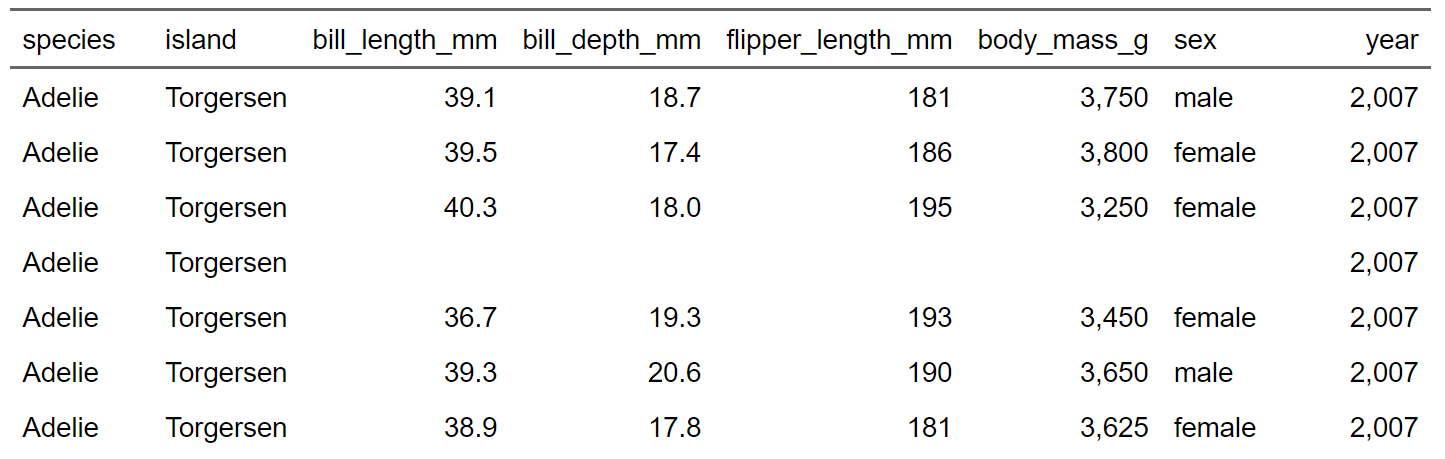
\includegraphics[width=\textwidth]{IMG/T1.png}
		\caption{Base de datos de los pingüinos palmer (primeros 5 casos)}
		\label{fig:f1}
	\end{minipage}\hfill
\end{figure}

La base esta compuesta por 344 observaciones y 8 variables (4 variables categóricas o de etiqueta y 4 variables numéricas continuas). Para efectos del desarrollo del documento, se tomaran en cuenta unicamente las 4 variables numéricas continuas (bill\_length, bill\_depth, flipper\_length y body\_mass) junto con la variable categórica de species para hacer el coloreado en los gráficos.

\newpage

La problemática que se desea abordar y  por la cual se quiere aplicar LDA es la siguiente: Se desea poder proyectar la información de las 4 dimensiones en un espacio de menor dimensionalidad, esto con la finalidad de poder observar gráficamente como se están comportando los datos.

Dada la naturaleza del LDA que es capaz de representar los datos en $k-1$ dimensiones, donde $k$ es la cantidad de grupos (en este caso, especies de pingüinos), se plantea el proyectar las aproximaciones en 1D y en 2D para el caso donde se tienen unicamente 2 especies y para el caso donde se tienen 3 especies respectivamente.

Con el objetivo de evidenciar lo difícil que es ver como se están comportando los datos a continuación se muestran los gráficos de dispersión tomando subconjuntos de las variables:

\begin{figure}[h!]
	\centering
	\begin{minipage}{1.1\textwidth}
		\centering
		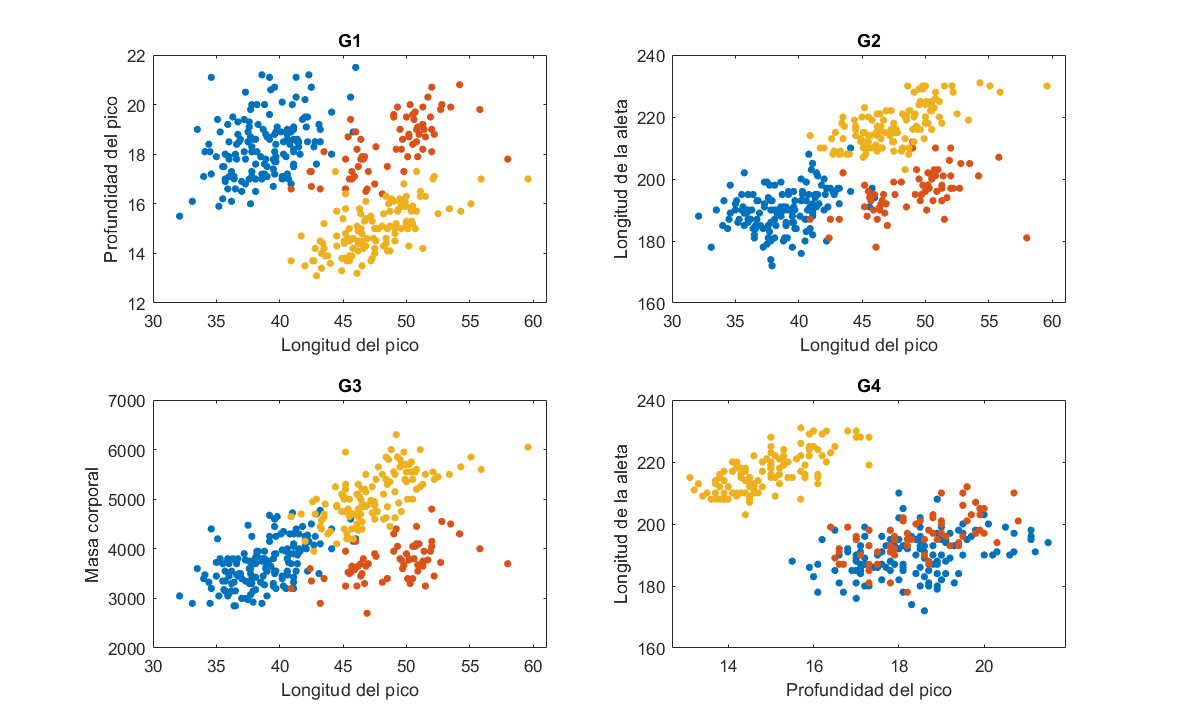
\includegraphics[width=\textwidth]{IMG/G1.png}
		\caption{Gráficos de dispersión bivariados.}
		\label{fig:f2}
	\end{minipage}\hfill
\end{figure}

Se puede observar que para algunos pares de variables, se alcanza a ver una separación clara de los datos por especies, sin embargo, al verlo desde otro par de variables, la cosa se vuelve difusa de distinguir, como es el caso del gráfico G4, en donde se esta mostrando el comportamiento de las variables de la profundidad del pico y el largo de la aleta.

\newpage

Por otro lado, se hizo la propuesta de modelarlos en 3 dimensiones, para observar como se comportan los datos en el espacio:

\begin{figure}[h!]
	\centering
	\begin{minipage}{1.1\textwidth}
		\centering
		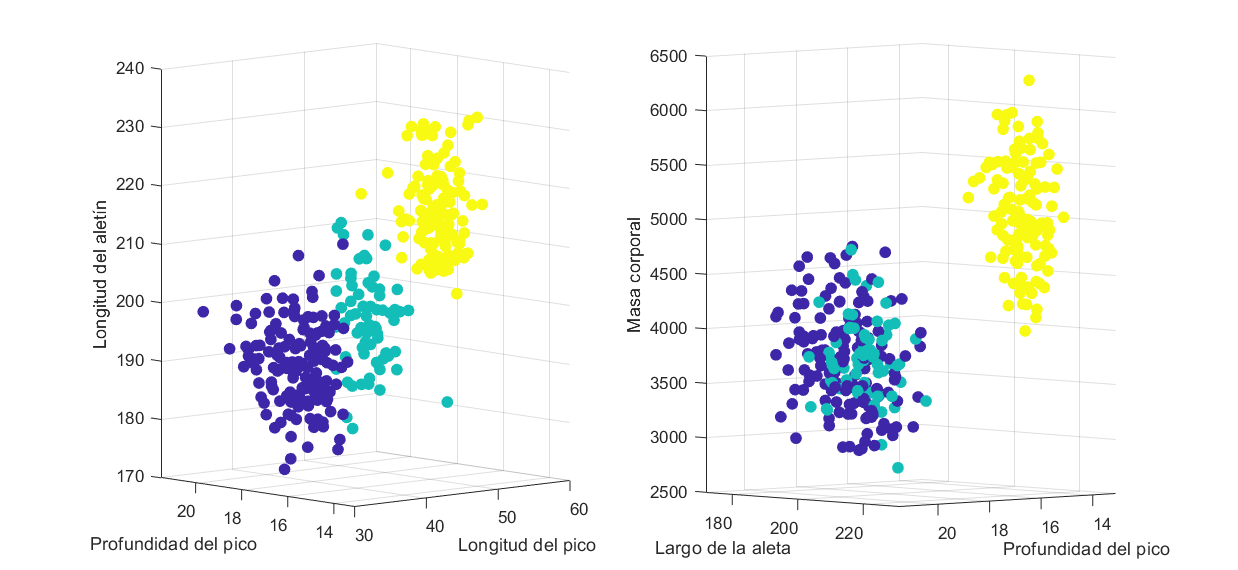
\includegraphics[width=\textwidth]{IMG/G2.png}
		\caption{Gráficos de dispersión multivariados.}
		\label{fig:f3}
	\end{minipage}\hfill
\end{figure}


En el primer gráfico se logra apreciar una separación distinguible entre los grupos de pingüinos dada su visualización mediante las variables de profundidad del pico, longitud del pico y longitud de la aleta. Por otro lado, en el gráfico de la derecha, se observa como un grupo esta perfectamente diferenciado del resto pero los 2 grupos restantes se encuentran sobre puestos uno con el otro, lo que los hace difíciles de separar usando las variables de profundidad del pico, largo de la aleta y masa corporal.

Es por ello que se quiere usar LDA para proyectar la información y reducir la dimensionalidad de los datos para observar mejor su comportamiento en 1 y 2 dimensiones.

	
	\newpage
	
	\section{Metodología}
	
	Para realizar el calculo del LDA  es necesario desglosarlo en varios pasos. Primero, cabe mencionar que el discriminante lineal es una técnica multivariada de aprendizaje supervisado que permite reducir la dimensionalidad de datos cuantitativos continuos que se encuentren etiquetados por una variable de clase, donde el resultado son $k-1$ combinaciones lineales donde proyectar los datos \cite{johnson2007}. 
	
	Para ejecutar la técnica, es necesario tener identificados a la matriz de caracteristicas $X$ y al vector de etiquetas o clases $Y$: 
	
	$$
	 \begin{matrix}
	 	X = \{x_1,x_2,\dots,x_n\} \\
	 	Y = \{Y_1, Y_2,\dots ,Y_k\}
	 \end{matrix}
	$$
	Donde: 
	\begin{itemize}
		\item $X$ Es la matriz de datos de tamaño $N\times P$.
		\item $Y$ Es el vector que contiene las clases de tamaño $N\times 1 $.
	\end{itemize}
	

Una vez identificados los elementos fundamentales para dar inicio a la técnica, se procede a calcular la matriz de dispersión entre clases como sigue:

$$S_w = \sum_{i = 1}^{k} {(X_i-\mu_i)(X_i-\mu_i)' }$$

	Donde: 
	\begin{itemize}
		\item $S_w$ Es la matriz de dispersión entre clases de tamaño $P\times P$.
		\item $X_i$ Es la matriz de de características $X$ de la clase $i$-ésima de tamaño $N_i \times P$.
		\item $\mu_i$ Es el vector de medias de la matrix $X_i$ de tamaño $1\times P$.
		\item $k$ Es la cantidad de clases en el conjunto de datos.
	\end{itemize}

\newpage

Posteriormente, se procede a calcular la dispersión total presente en los datos como sigue:

$$S_t = {(X-\mu)(X-\mu)' }$$

Donde: 
\begin{itemize}
	\item $S_t$ Es la matriz de dispersión de todo el conjunto de datos sin considerar clases de tamaño $P\times P$.
	\item $X$ Es la matriz de de características $X$ de tamaño $N \times P$.
	\item $\mu$ Es el vector de medias de la matrix $X$ de tamaño $1\times P$.
\end{itemize}

Una vez hecho el calculo de la matriz de dispersión global $S_t$, se obtiene por diferencia la matriz de dispersión dentro de clases como sigue:

$$S_b = S_t-S_w$$

Donde: 

\begin{itemize}
	\item $S_b$ Es la matriz de dispersión entre clases de tamaño $P\times P$.
	\item $S_t$ Es la matriz de de dispersión de los datos de tamaño $P \times P$.
	\item $S_w$ Es la matriz de de dispersión dentro de clases de tamaño $P \times P$.
\end{itemize}

Una vez determinadas las matrices de dispersión entre clases y dentro de clases, el siguiente paso es maximizar el criterio de Fisher, el cual busca que las clases esten lo más separadas posibles y que la varianza dentro de las clases sea la más pequeña posible como se muestra a continuación:

$$MAX \quad J(W)  = \frac{|W^TS_bW|}{|W^TS_wW|}$$

Donde: 

\begin{itemize}
	\item $J(W)$ Es el criterio de Fisher.
	\item $W$ Es la matriz de vectores propios de tamaño $P \times P$.
	\item $S_b$ Es la matriz de dispersión entre clases de tamaño $P\times P$.
	\item $S_w$ Es la matriz de de dispersión dentro de clases de tamaño $P \times P$
\end{itemize}

\newpage

Para encontrar los valores de la matriz $W$ que logran maximizar el criterio de fisher, se resuelve como un problema de valores propios generalizados como se muestra:

$$S_bW = \lambda S_wW$$

Donde: 

\begin{itemize}
	\item $W$ Es la matriz de vectores propios de tamaño $P \times P$.
	\item $S_b$ Es la matriz de dispersión entre clases de tamaño $P\times P$.
	\item $S_w$ Es la matriz de de dispersión dentro de clases de tamaño $P \times P$
	\item $\lambda$ Es el vector de valores propios de tamaño $1 \times P$.
\end{itemize}

El resultado esperado son $P$ valores propios que indican cuanta varianza acumula cada una de las componentes en el nuevo sistema de coordenadas donde se van a proyectar los datos originales y $P$ vectores propios que serán los ejes sobre los cuales se proyecten los datos.

Para hacer la proyección de los datos centrados en el nuevo sistema, basta con aplicar la siguiente operación matricial con los vectores propios encontrados:

$$Z = XW$$

Donde: 
\begin{itemize}
	\item $Z$ Son las proyecciones de las características X sobre los vectores W.
	\item $X$ Es la matriz de características de tamaño $N \times P$.
	\item $W$ es la matriz de vectores propios de tamaño $P \times P$ .
\end{itemize}

Finalmente, se calcula la variabilidad explicada por cada componente mediante los valores propios como sigue:

$$VE = 100*\frac{\lambda_i}{\sum_{i = 1}^P{\lambda_i}}$$

Donde: 
\begin{itemize}
	\item $VE$ Es la variabilidad explicada por el $i$-ésimo valor propio.
	\item $\lambda_i$ Es el $i$-ésimo valor propio.
\end{itemize}

Cabe mencionar que los valores propios conservan la siguiente propiedad:

$$\lambda_1 \geq \lambda_2 \geq \dots \geq \lambda_P$$

Nota importante: Debido a que el discriminante lineal toma en cuenta la cantidad de clases con las que se esta trabajando, logra reducir aun más el número de dimensiones tal que solo se van a proyectar $k-1$ dimensiones como resultado.
Pese a que operativamente se generen $P$ valores y vectores propios, la realidad es que solo $k-1$ valores propios van a ser distintos de 0, esto implica que los  vectores propios asociados a esos $k-1$ valores propios distintos de 0 van a ser los proyectados y que concentran la información original en una menor dimensionalidad.

Como ejemplo, si se tienen 2 clases y 4 variables, el sistema va a calcular 4 valores propios y 4 vectores propios, pero solo $2-1$ valores propios van a ser distintos de 0, por lo que toda la variabilidad explicada recae en un solo vector propio, por lo que la salida de los datos sera su proyección en 1 dimensión.

Otro ejemplo, si se tienen 3 clases y 4 variables, el sistema va a calcular 4 valores propios y 4 vectores propios, pero solo $3-1$ valores propios van a ser distintos de 0, por lo que toda la variabilidad explicada recae en dos vectores propios, por lo que la salida de los datos sera su proyección en 2 dimensiones.

\newpage

A continuación, se aplico un breve pre-procesamiento de los datos:

- Se identificaron y eliminaron las filas con valores faltantes (2 filas eliminadas)
- Se guardo en $X$  las variables numéricas de longitud del pico, profundidad del pico, largo de la aleta y masa corporal.
- Se guardo en $Y$ las etiquetas de la especie a la que pertenecen los individuos.

Posteriormente, se aplico LDA para reducir dimensionalidad en 2 casos: para los datos recortados unicamente con 2 especies de pingüinos (Adelie y Chinstrap) y para el caso de la base de datos completa que contempla las 3 especies de pingüinos (Adelie, Chinstrap y Gentoo).
	
\newpage
	
\section{Resultados para dos clases}

A continuación se muestran los resultados obtenidos para los datos de los pingüinos palmer en matlab cuando se trabajan con 2 clases. 

\subsection{Vectores de medias}

Se muestra el vector de medias obtenido para las variables de Longitud del pico, profundidad del pico, longitud de la aleta y la masa corporal para la especie Adelie, Chinstrap y el vector de medias general:

$$
\begin{matrix}
	\mu_{Adelie} =  &\{38.7914 & 18.3464 & 189.9536 & 3700.662\}	 \\
	\mu_{Chinstrap} = & \{48.8338 & 18.4206 & 195.8235 & 3733.088\}	 \\
	\mu = & \{41.90959 & 18.36941 & 191.77626 & 3710.73059 \}	 
\end{matrix}
$$


Se observa la evidente diferencia de las escalas entre las variables, siendo la masa corporal la que tiene valores más altos respecto al resto de variables.

\subsection{Matriz de dispersión dentro de clases}

Aplicando la definición para la matriz de dispersión dentro de las clases descrita previamente, se obtuvo la siguiente matriz:

$$
S_w = 
\begin{bmatrix}
1811.1510 & 356.3029 & 1603.6456 & 144719.76\\
356.3029 & 308.4067 & 681.8716 & 65889.04\\
1603.6456 & 681.8716 & 9822.5578 & 328426.69\\
144719.7580 & 65889.0407 & 328426.6946 & 41439235.25
\end{bmatrix}
$$

\newpage

\subsection{Matriz de dispersión entre clases}

Aplicando la definición para la matriz de dispersión entre las clases descrita previamente, se obtuvieron las siguientes matrices (la matriz de dispersión global y la matriz de dispersión entre clases):

$$
S_t = 
\begin{bmatrix}
	6539.6099 & 391.2542 & 4367.4699 & 159987.5 \\
	391.2542 & 308.6650 & 702.3009 & 66001.9 \\
	4367.4699 & 702.3009 & 11438.0365 & 337350.8 \\
	159987.4658 & 66001.8950 & 337350.7991 & 41488533.1
\end{bmatrix}
$$

$$
S_b = S_t-S_w = 
\begin{bmatrix}
4728.4588 & 34.9513 & 2763.8242 & 15267.7078 \\
34.9513 & 0.2583 & 20.4294 & 112.8543 \\
2763.8242 & 20.4294 & 1615.4787 & 8924.1045 \\
15267.7078 & 112.8543 & 8924.1045 & 49297.8596
\end{bmatrix}
$$

\newpage


\subsection{Valores y vectores propios}

Se construye la matriz que representa el criterio de Fisher a Maximizar:

$$S = S_w^{-1}S_b = 
\begin{bmatrix}
3.7501 & 0.0277 & 2.1919 & 12.1085 \\
-2.4144 & -0.0178 & -1.4112 & -7.7957 \\
0.1823 & 0.0013 & 0.1065 & 0.5885 \\
-0.0103 & -0.0001 & -0.0060 & -0.0334
\end{bmatrix}
$$

Posteriormente, se calculan los valores y vectores propios como resultado de la resolución de la matriz S como un problema de valores y vectores propios generalizado como sigue:

$$\lambda = 
\begin{bmatrix}
	3.8054 &
	0 &
	0 &
	0 
\end{bmatrix}
$$

$$ W = 
\begin{bmatrix}
0.8401 & 0.2773 & -0.0506 & -0.0018 \\
-0.5409 & 0.8034 & -0.9958 & -1.0000 \\
0.0408 & -0.5268 & 0.0766 & 0.0085 \\
-0.0023 & 0.0076 & 0.0041 & 0.0013
\end{bmatrix}
$$

Se observa como el valor asociado a la variable de masa corporal en el primer vector propio es el que tiene un mayor peso en la primer componente, siendo así mismo que la longitud de la aleta tiene mayor peso sobre la componente 2, la componente 3 se caracteriza porque su mayor peso recae en la variable de longitud del pico y la variable 4 indica que el mayor peso recae sobre la variable de la profundidad del pico.

Haciendo las cuentas, a continuación se muestra cuanta variabilidad explica cada componente:

$$VE = 
\begin{bmatrix}
	100 &
	0 &
	0 &
	0 
\end{bmatrix}
$$



Se observa como más del 99\% de la variabilidad explicada recae sobre el primer componente.


\newpage

\subsection{Proyección de las nuevas componentes}

A continuación se muestra una pequeña fracción de los datos al ser proyectados sobre el nuevo sistema creado con ayuda de los vectores propios:

\begin{figure}[h!]
	\centering
	\begin{minipage}{0.8\textwidth}
		\centering
		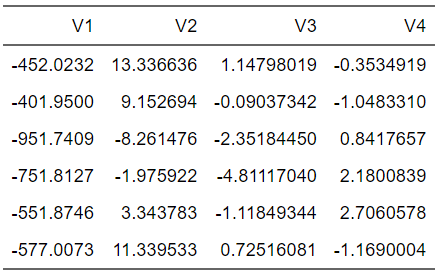
\includegraphics[width=0.3\textwidth]{IMG/T2.png}
		\caption{Base de datos centrada y proyectada sobre los vectores propios (primeros 5 casos).}
		\label{fig:f4}
	\end{minipage}\hfill
\end{figure}

Se observa como los valores más grandes de los valores proyectados se encuentran entre las componentes 1 y 2.

\newpage

\subsection{Proyección en 1D}

Debido al sorprendente resultado que indica que el 99\% de la variabilidad de los datos recae sobre la primer componente, se decidió probar a graficar la primer componente en un gráfico de puntos unidimensional. El resultado fue el siguiente:

\begin{figure}[h!]
	\centering
	\begin{minipage}{1.1\textwidth}
		\centering
		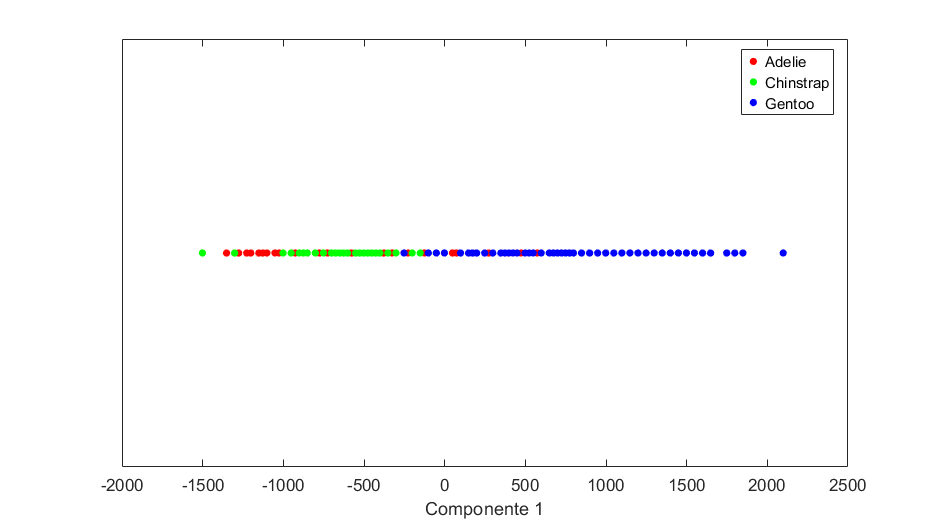
\includegraphics[width=\textwidth]{IMG/G3.png}
		\caption{Proyección en 1D sobre el componente 1.}
		\label{fig:f5}
	\end{minipage}\hfill
\end{figure}

El gráfico muestra la proyección de los datos en un espacio unidimensional, donde se observa que la mitad derecha esta mayormente representada por pingüinos de la especie Gentoo, mientras que la mitad izquierda presenta el problema del traslape entre clases. Pese a que la varianza explicada sea del 99\%, no se puede interpretar mucho a simple vista.

\newpage

\section{Resultados para tres clases}

A continuación se muestran los resultados obtenidos para los datos de los pingüinos palmer en matlab cuando se trabajan con las 3 clases del conjunto de datos. 

\subsection{Vectores de medias}

Se muestra el vector de medias obtenido para las variables de Longitud del pico, profundidad del pico, longitud de la aleta y la masa corporal para la especie Adelie, Chinstrap, Gentoo y el vector de medias general:

$$
\begin{matrix}
	\mu_{Adelie} =  &\{38.7914 & 18.3464 & 189.9536 & 3700.662\}	 \\
	\mu_{Chinstrap} = & \{48.8338 & 18.4206 & 195.8235 & 3733.088\}	 \\
	\mu_{Gentoo} = & \{47.5049 & 14.9821 &  217.1870  & 5076.016\}	 \\
	\mu = & \{43.9219 & 17.1512 & 200.9152 & 4201.7544 \}	 
\end{matrix}
$$



Se observa la evidente diferencia de las escalas entre las variables, siendo la masa corporal la que tiene valores más altos respecto al resto de variables.

\subsection{Matriz de dispersión dentro de clases}

Aplicando la definición para la matriz de dispersión dentro de las clases descrita previamente, se obtuvo la siguiente matriz:

$$
S_w = 
\begin{bmatrix}
2969.8881 & 593.6636 & 3215.733 & 271554.1 \\
593.6636 & 425.8673 & 1230.383 & 109283.8 \\
3215.7334 & 1230.3829 & 14953.257 & 608678.3 \\
271554.1482 & 109283.7765 & 608678.321 & 72443483.2
\end{bmatrix}
$$

\newpage

\subsection{Matriz de dispersión entre clases}

Aplicando la definición para la matriz de dispersión entre las clases descrita previamente, se obtuvieron las siguientes matrices (la matriz de dispersión global y la matriz de dispersión entre clases):

$$
S_t = 
\begin{bmatrix}
10164.2055 & -864.1738 & 17178.136 & 888506.8 \\
-864.1738 & 1329.8345 & -5528.616 & -254853.2 \\
17178.1360 & -5528.6161 & 67426.541 & 3350125.9 \\
888506.8421 & -254853.2018 & 3350125.877 & 219307697.4
\end{bmatrix}
$$

$$
S_b = S_t-S_w = 
\begin{bmatrix}
7194.317 & -1457.8374 & 13962.403 & 616952.7 \\
-1457.837 & 903.9672 & -6758.999 & -364137.0 \\
13962.403 & -6758.9990 & 52473.284 & 2741447.6 \\
616952.694 & -364136.9782 & 2741447.557 & 146864214.2
\end{bmatrix}
$$

\newpage


\subsection{Valores y vectores propios}

Se construye la matriz que representa el criterio de Fisher a Maximizar:

$$S = S_w^{-1}S_b = 
\begin{bmatrix}
3.2165 & -0.4000 & 4.6163 & 176.8832 \\
-12.5988 & 6.5009 & -49.9444 & -2631.6653 \\
0.9866 & -0.5443 & 4.1384 & 219.9163 \\
0.0072 & -0.0088 & 0.0611 & 3.4865
\end{bmatrix}
$$

Posteriormente, se calculan los valores y vectores propios como resultado de la resolución de la matriz S como un problema de valores y vectores propios generalizado como sigue:

$$\lambda = 
\begin{bmatrix}
	15.0192 &
	2.3231 &
	0 &
	0 
\end{bmatrix}
$$

$$ W = 
\begin{bmatrix}
-0.0846 & -0.9982 & -0.0375 & 0.2808 \\
0.9930 & -0.0502 & -0.9943 & -0.8166 \\
-0.0825 & 0.0322 & 0.0997 & -0.5043 \\
-0.0012 & 0.0041 & -0.0042 & 0.0062
\end{bmatrix}
$$

Se observa como el valor asociado a la variable de masa corporal en el primer vector propio es el que tiene un mayor peso en la primer componente, siendo así mismo que la longitud de la aleta tiene mayor peso sobre la componente 2, la componente 3 se caracteriza porque su mayor peso recae en la variable de longitud del pico y la variable 4 indica que el mayor peso recae sobre la variable de la profundidad del pico.

Haciendo las cuentas, a continuación se muestra cuanta variabilidad explica cada componente:

$$VE = 
\begin{bmatrix}
	86.6046  &
	13.3954  &
	0 &
	0 
\end{bmatrix}
$$



Se observa como más del 99\% de la variabilidad explicada recae sobre el primer componente.


\newpage

\subsection{Proyección de las nuevas componentes}

A continuación se muestra una pequeña fracción de los datos al ser proyectados sobre el nuevo sistema creado con ayuda de los vectores propios:

\begin{figure}[h!]
	\centering
	\begin{minipage}{0.8\textwidth}
		\centering
		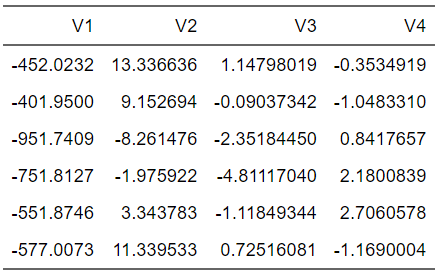
\includegraphics[width=0.3\textwidth]{IMG/T2.png}
		\caption{Base de datos centrada y proyectada sobre los vectores propios (primeros 5 casos).}
		\label{fig:f6}
	\end{minipage}\hfill
\end{figure}

Se observa como los valores más grandes de los valores proyectados se encuentran entre las componentes 1 y 2.

\newpage

\subsection{Proyección en 1D}

Debido al sorprendente resultado que indica que el 99\% de la variabilidad de los datos recae sobre la primer componente, se decidió probar a graficar la primer componente en un gráfico de puntos unidimensional. El resultado fue el siguiente:

\begin{figure}[h!]
	\centering
	\begin{minipage}{1.1\textwidth}
		\centering
		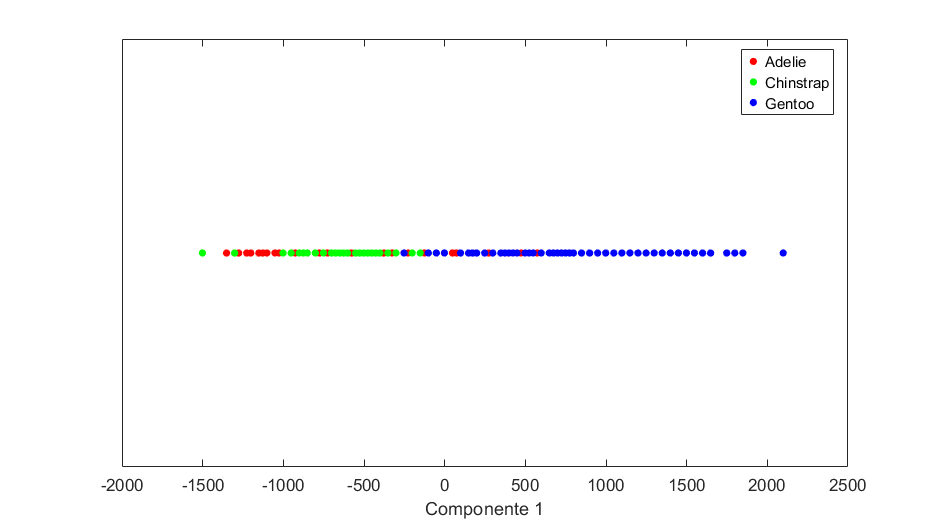
\includegraphics[width=\textwidth]{IMG/G3.png}
		\caption{Proyección en 1D sobre el componente 1.}
		\label{fig:f7}
	\end{minipage}\hfill
\end{figure}

El gráfico muestra la proyección de los datos en un espacio unidimensional, donde se observa que la mitad derecha esta mayormente representada por pingüinos de la especie Gentoo, mientras que la mitad izquierda presenta el problema del traslape entre clases. Pese a que la varianza explicada sea del 99\%, no se puede interpretar mucho a simple vista.




\newpage
	
\section{Conclusiones}
	
Después de realizar el ejercicio de explorar una base de datos y aplicarle PCA para poder proyectar su información concentrada en un espacio de menor dimensionalidad, se pudo observar como el PCA mejora sustancialmente la representación de los datos al poder comprimir las variables en un espacio de menor dimensionalidad sin perder apenas información.

La técnica es eficaz, relativamente simple y bastante potente, aunque presenta algunas debilidades. Una de las principales es su sensibilidad a la escala de las variables. Como se observó en el ejercicio, la variable masa corporal, que tenía los valores más grandes, resultó ser la que más aportó a la primera componente principal. Esto se debe a que, al tener mayor variabilidad absoluta, influye más en el cálculo de los valores propios, lo que provoca que se le atribuya una mayor capacidad explicativa. Para enfrentar este tipo de situaciones, se recomienda estandarizar los datos mediante una transformación $Z$, o bien utilizar la matriz de correlaciones en lugar de la matriz de covarianzas.

El otro problema que acarrea consigo el PCA es la posibilidad de que la matriz de varianzas y covarianzas o la de correlaciones (cualquiera que se este usando) tenga la particularidad de ser NO invertible, por lo que ahí la técnica ya no es posible aplicarla.

Más allá de estos problemas, la técnica probo ser buena para mejorar la visualización de los datos para este caso de aplicación.

\newpage

	
\section{Referencias}  % Sección numerada de referencias
\bibliographystyle{apalike}  % Estilo de citas (puedes cambiarlo)
\bibliography{Biblio}        % Nombre del archivo BibTeX (sin extensión)

\newpage
	
\section{Anexos}	
\subsection{Implementación de la exploración y el PCA en MATLAB}
\begin{minted}[linenos,firstnumber=1]{matlab}
%% Cargar la base de datos en formato CSV %%
ruta = "penguins.csv";
datos = readtable(ruta); % Leer el archivo CSV en una tabla
size(datos); % Ver el tamaño de los datos

% 1 etiqueta de clasificación (Species)
% 3 características categóricas (Isla, sexo y año de observación)
% 4 variables continuas: bill length, bill depth, fliper y bodymass

% Filtrar solo las columnas numéricas y eliminar filas con datos faltantes
indices = find(any(isnan(datos{:, 4:7}), 2)); % Buscar filas con valores NaN en las columnas 4 a 7
datos1 = datos;
datos1(indices, :) = []; % Eliminar esas filas

% Extraer las variables numéricas y la especie para el gráfico
% Extraer las variables numéricas y la especie para el gráfico
especie = datos1.species; % Columna 'species' con las etiquetas de especies
% Convertir la columna 'especie' en un vector de tipo categorical
especie = categorical(especie); % Convertir a tipo categorical, que gscatter entiende
datos1 = table2array(datos1(:, 4:7)); % Convertir las columnas 4 a 7 a un arreglo numérico

%% Gráficos descriptivos %%
% Graficar el gráfico de dispersión usando gscatter
% Longitud del pico y ancho del pico
subplot(2,2,1)
gscatter(datos1(:,1), datos1(:,2), especie,"filled"); 
xlabel('Longitud del pico'); % Etiqueta del eje x
ylabel('Profundidad del pico'); % Etiqueta del eje y
title('G1'); % Título del gráfico

% Longitud del pico y longitud de la aleta %
subplot(2,2,2)
gscatter(datos1(:,1), datos1(:,3), especie,"filled");
xlabel('Longitud del pico'); % Etiqueta del eje x
ylabel('Longitud de la aleta'); % Etiqueta del eje y
title('G2'); % Título del gráfico
% Longitud del pico y masa corporal
subplot(2,2,3)
gscatter(datos1(:,1), datos1(:,4), especie,"filled");
xlabel('Longitud del pico'); % Etiqueta del eje x
ylabel('Masa corporal'); % Etiqueta del eje y
title('G3'); % Título del gráfico
% Ancho del pico y Longitud de la aleta
subplot(2,2,4)
gscatter(datos1(:,2), datos1(:,3), especie,"filled");
xlabel('Profundidad del pico'); % Etiqueta del eje x
ylabel('Longitud de la aleta'); % Etiqueta del eje y
title('G4'); % Título del gráfico

%% Exploración en 3D %&
% Crear un gráfico 3D
subplot(1,2,1)
scatter3(datos1(:,1), datos1(:,2), datos1(:,3), 50, especie, 'filled'); 
% Ajustar etiquetas y título
xlabel('Longitud del pico');
ylabel('Profundidad del pico');
zlabel('Longitud del aletín');
title('');

subplot(1,2,2)
scatter3(datos1(:,2), datos1(:,3), datos1(:,4), 50, especie, 'filled'); 
% Ajustar etiquetas y título
xlabel('Profundidad del pico');
ylabel('Largo de la aleta');
zlabel('Masa corporal');
title('');
% Mostrar la leyenda de colores
% Guardar como archivo PNG

%% HACER EL PCA %%

% Obtener la media de los datos
%% Cambio de coordenadas %%
medias = mean(datos1)
cdatos = datos1 - medias % Centrar en la media


% Calculo de la covarianza %
n = size(datos1);
Si = (cdatos'*cdatos)/(n(1)-1)

%% Calcular los eigen valores %%
[V, D] = eig(Si)

100*diag(D)/sum(diag(D))

%% Calcular los scores %%
%% Calcular los scores %%
NB = cdatos * V; % Proyección de los datos

% Crear una dispersión en 1D (todos los puntos con la misma Y)
y = zeros(size(NB, 1), 1); % Todos los puntos en Y=0
gscatter(NB(:,4), y, especie, 'rgb', '.', 15);
xlabel('Componente 1');
yticks([]); % Eliminar marcas del eje Y
ylabel('');
title('Proyección 1D sobre el componente 1');

%% Gráfico en 2d con la primer y segunda componente %%
gscatter(NB(:,4), NB(:,3), especie,"filled");
xlabel('Componente 1'); % Etiqueta del eje x
ylabel('Componente 2'); % Etiqueta del eje y
title(''); % Título del gráfico

%% Crear un gráfico 3D %%
scatter3(NB(:,4), NB(:,3), NB(:,2), 50, especie, 'filled'); 
% Ajustar etiquetas y título
xlabel('Componente 1');
ylabel('Componente 2');
zlabel('Componente 3');
title('');
\end{minted}
	
	
	
	
\end{document}

